    In order to study the impact of regional disaster, we augment a standard AS logical connectivity graph~\cite{caida-asgraph} with measurements of the geographic regions in which networks peer.
    We model the Earth as a geodesic globe inscribed in a sphere of the Earth's radius, and map latitude and longitude values to a face on the globe.
    We consider each face of the globe as a `region,' such that a worst-case disaster could destroy all of the physical routing infrastructure within the region.
    We generate the geodesic globe using a standard algorithm~\cite{geodesic}, providing us with 327,680 triangular faces, each with average side length of \shaddi{m km} and area \shaddi{n km$^2$}.  
    Finally, we map locations where ASes peer to faces on the globe.
    The same technique could be applied to intradomain connectivity for large networks, but we leave this analysis to future work.    
 
    We develop our peering dataset by borrowing techniques and data from
    the IXP
    Mapping Project~\cite{ixps-mapped}, iPlane~\cite{iplane},
    Aqualab~\cite{sidewalk},
    CAIDA~\cite{caidadata}, and the MaxMind~\cite{maxmind} industrial IP geolocation service.
    For the iPlane and Aqualab data, we derive peering points from raw traceroute files.
    For each pair of IP addresses we observe adjacent in a traceroute, we map the IPs to alias clusters generated by CAIDA's iffinder~\cite{iffinder} and MIDAR~\cite{iffinder, midar} measurements.
    We then map the alias clusters to ASes, and if the ASes are different, we store the two IP addresses as an AS peering.
    We map the peering to a geographic location using a combination of DNS-based geolocation and the MaxMind commercial geolocation service.
    For both IP addresses in the adjacency, we do reverse DNS lookups on all IP addresses in their alias clusters. 
    If any of the DNS names match rules from the undns~\cite{undns} or sarang~\cite{sarang} projects, we map the IP address to that location. 
    If multiple of the IP addresses point to different locations, we elect the most common location, or in a tie, choose the location with the least distance from the others.
    If no DNS names are found, we repeat the same process with locations from the MaxMind GeoLite City database, which has better coverage that DNS geolocation, but worse accuracy~\cite{uhlig_ccr_paper}. 
    
    The measurements we gathered from CAIDA, iPlane, and Aqualab allowed us to identify \justine{k} router-level AS adjacencies, which we mapped to \justine{p} unique latitude, longitude locations (\justine{f} using DNS, and a further \justine{g} using MaxMind). 
    We mapped these adjacencies to \justine{h} unique faces of the geodesic globe.   
 
    \justine{Should I write why not map exchange poinst here?}

        \subsubsection*{Evaluation of Model}
            \begin{itemize}
        \item survey random network providers and ask them if what we
        found was correct
        \item Compare iPLaney data to Brice (Manual) Data.
        \item compare physical links discovered to logical connectivity
        graph (CAIDA provides this) - what fraction of logical links
        did we observe? For Tier-1's? For Tier-2's? For stub networks?
            \end{itemize} 

\begin{figure}[tb]
\centering
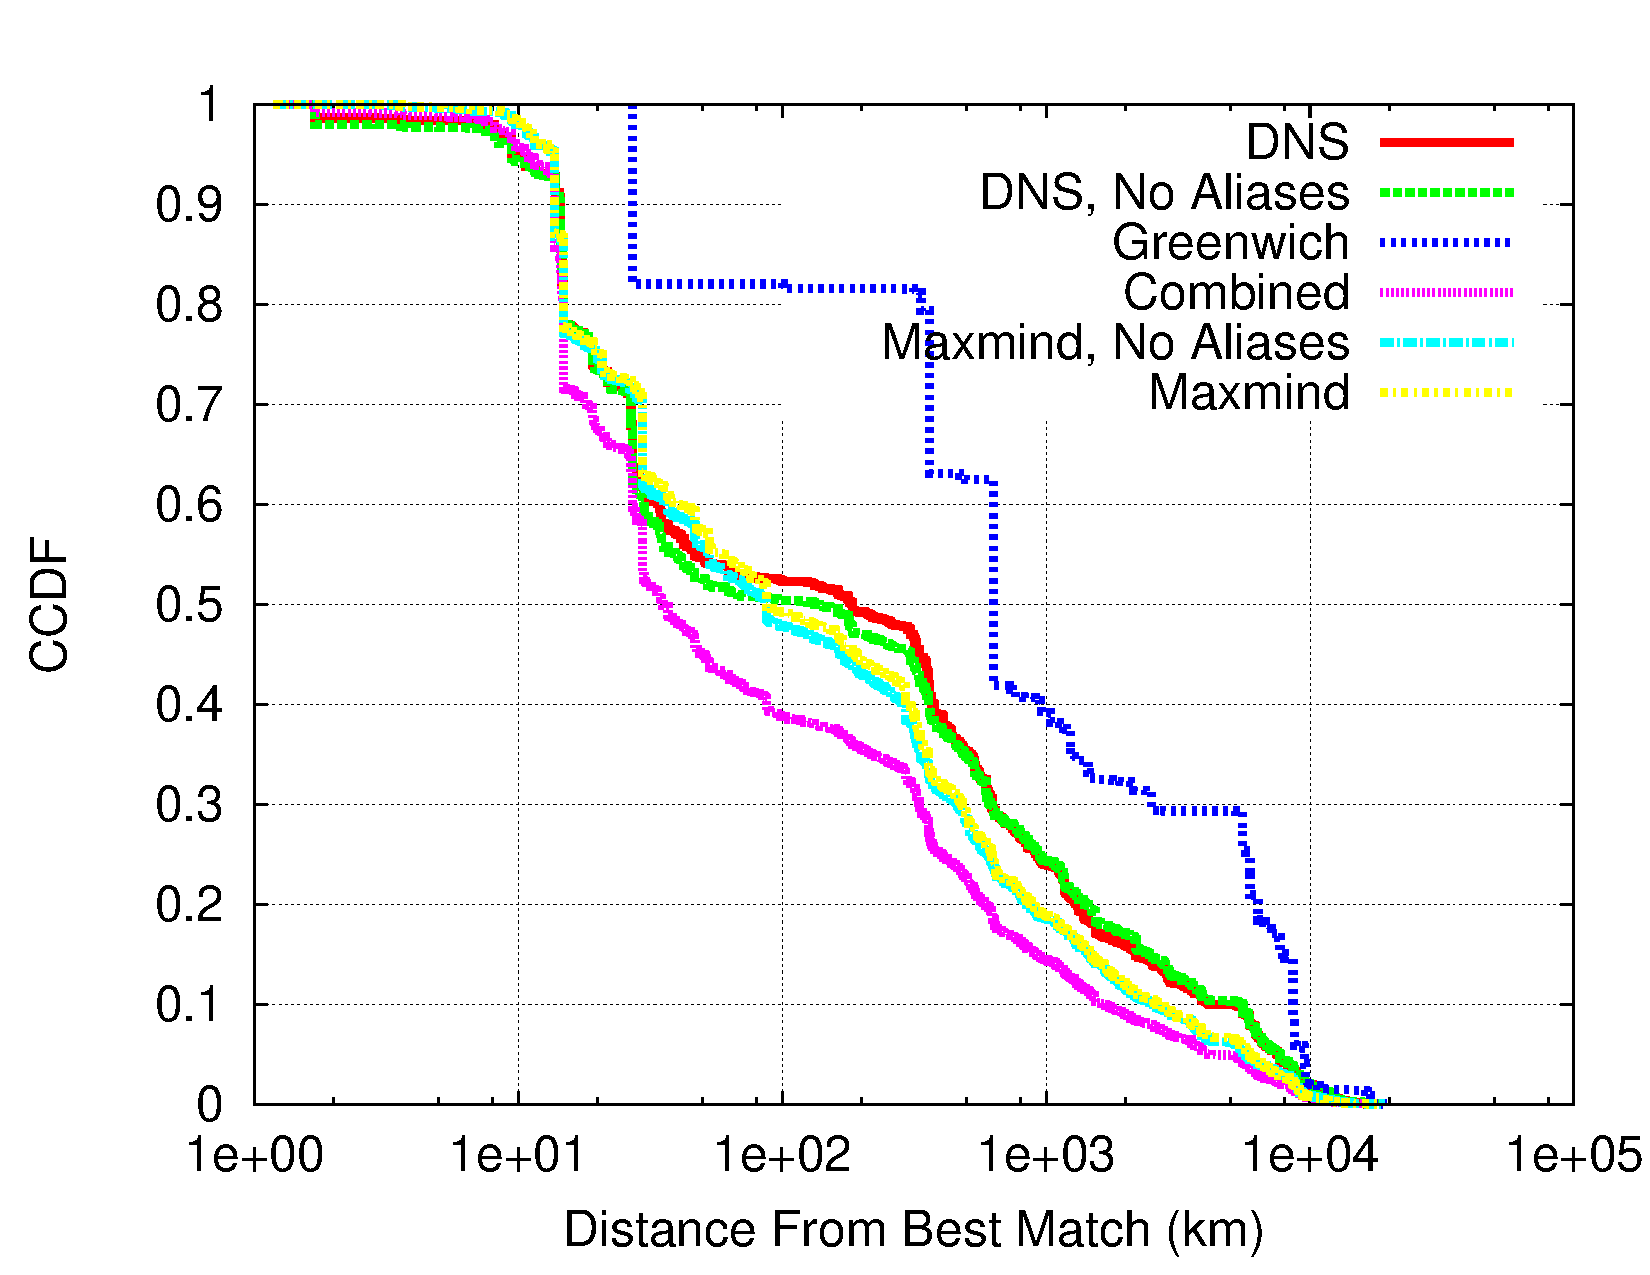
\includegraphics[width=3.25in]{graph_all_match_ccdf}
\caption[]{For ground truth peering locations, CCDF of distance to closest AS adjacency in our dataset using varying geolocation techniques. X-axis is in log scale.} 
%The $y$-axis is fraction of AS pairs with a path between them that traverses a service supporting AS. The $x$-axis is the fraction of ASes in the simulation topology supporting the service. }
%Using MIRO~\cite{miro} style multipath allows networks to provide access to services 
%even when their default path does not encounter a service-supporting AS.}
\end{figure}


